\documentclass[../algebraNotesMSRI-UP2016.tex]{subfiles}

\begin{document}

\section[\S \thesection]{Group homomorphisms}\label{sec:2p6groupHomomorphisms}
% % % % %
\subsection[\subsecname]{Definition}
% % %
\begin{frame}[c]{\subsecname}{}
%When its source and target have additional structure (e.g., the sets are groups, rings, vector spaces, etc.), a function that preserves the structure is called a \vocab{morphism}.  In our context, formally,
\begin{dfn}
A function $\varphi:(G,\star)\to(H,\bullet)$ between groups is called a \vocab{group homomorphism} means for every $g_1,g_2\in G$,
\[
\varphi(g_1\star g_2)=\varphi(g_1)\bullet\varphi(g_2).
\]
\end{dfn}

\smallGap
In other words, a group homomorphism keeps the group operation consistent between the source and the target.
\end{frame}

% % %
\begin{frame}
\begin{exe}[cf. Problem 62]\label{exe:detExample}
Which of the following are group homomorphisms? (What are the implied operations?)
\begin{enumerate}[(a)]
\item $\phi_1:\R\to \R$ via $\phi_1:a\mapsto a^2$
\item $\phi_2:\Q\to \Q$ via $\phi_2:a\mapsto a+10$
\item $\phi_3:\Z\to \Z$ via $\phi_3:a\mapsto 6a$.
\item\label{expt:detExampled} $\delta:\GL(2,\R)\to \R^{\times}$ via 
\[
\delta: \begin{pmatrix}
	a & b \\
	c & d 
	\end{pmatrix}
	\mapsto ad-bc.
\]
\end{enumerate}
\end{exe}
\end{frame}

% % % % %
\subsection[\subsecname]{Isomorphisms}\label{subsec:isomorphisms}
% % %
\begin{frame}{\subsecname}
Recall, from Section \ref{subsec:setsAndFunctions}, what it means for a function to be one-to-one (injective) or onto (surjective).

\smallGap
When a function is both injective and surjective, it is called \vocab{bijective}.  We say there is a \vocab{one-to-one correspondence} between the source and the target.

\smallGap  
\begin{dfn}
A bijective homomorphism is called an \vocab{isomorphism}.  The source and target are said to be \vocab{isomorphic}.
\end{dfn}

\smallGap
Exhibiting a group isomorphism demonstrates that the source and target are really the ``same" group, with different names.
\end{frame}

% % % 
\begin{frame}
\begin{ex}\label{ex:exponentialFunction}
Define the exponential function
\begin{align*}
E:(\R,+) &\to (\R^+,\cdot) \\
a &\mapsto e^a,
\end{align*}
where $\R^+$ denotes the set of positive real numbers and $e\approx 2.71928$ is the Euler number.  
\end{ex}
\smallGap
\textbf{Claim.} $E$ gives a bijection between $(\R,+)$ and $(\R^+,\cdot)$.  In other words, $(\R,+)$ and $(\R^+,\cdot)$ are isomorphic as groups, and we write: 
\[
(\R,+)\cong (\R^+,\cdot)
\]
\end{frame}

% % %
\begin{frame}{}{}
\pf When exhibiting an isomorphism, make sure to verify it is well-defined -- i.e., is $E:\R\to \R^+$ truly a group homomorphism?
\begin{itemize}
\item Recall, from Precalculus courses, the exponential function is always positive and passes the ``vertical line test" (see the figure below).  So $E$ is a function.

\begin{center}
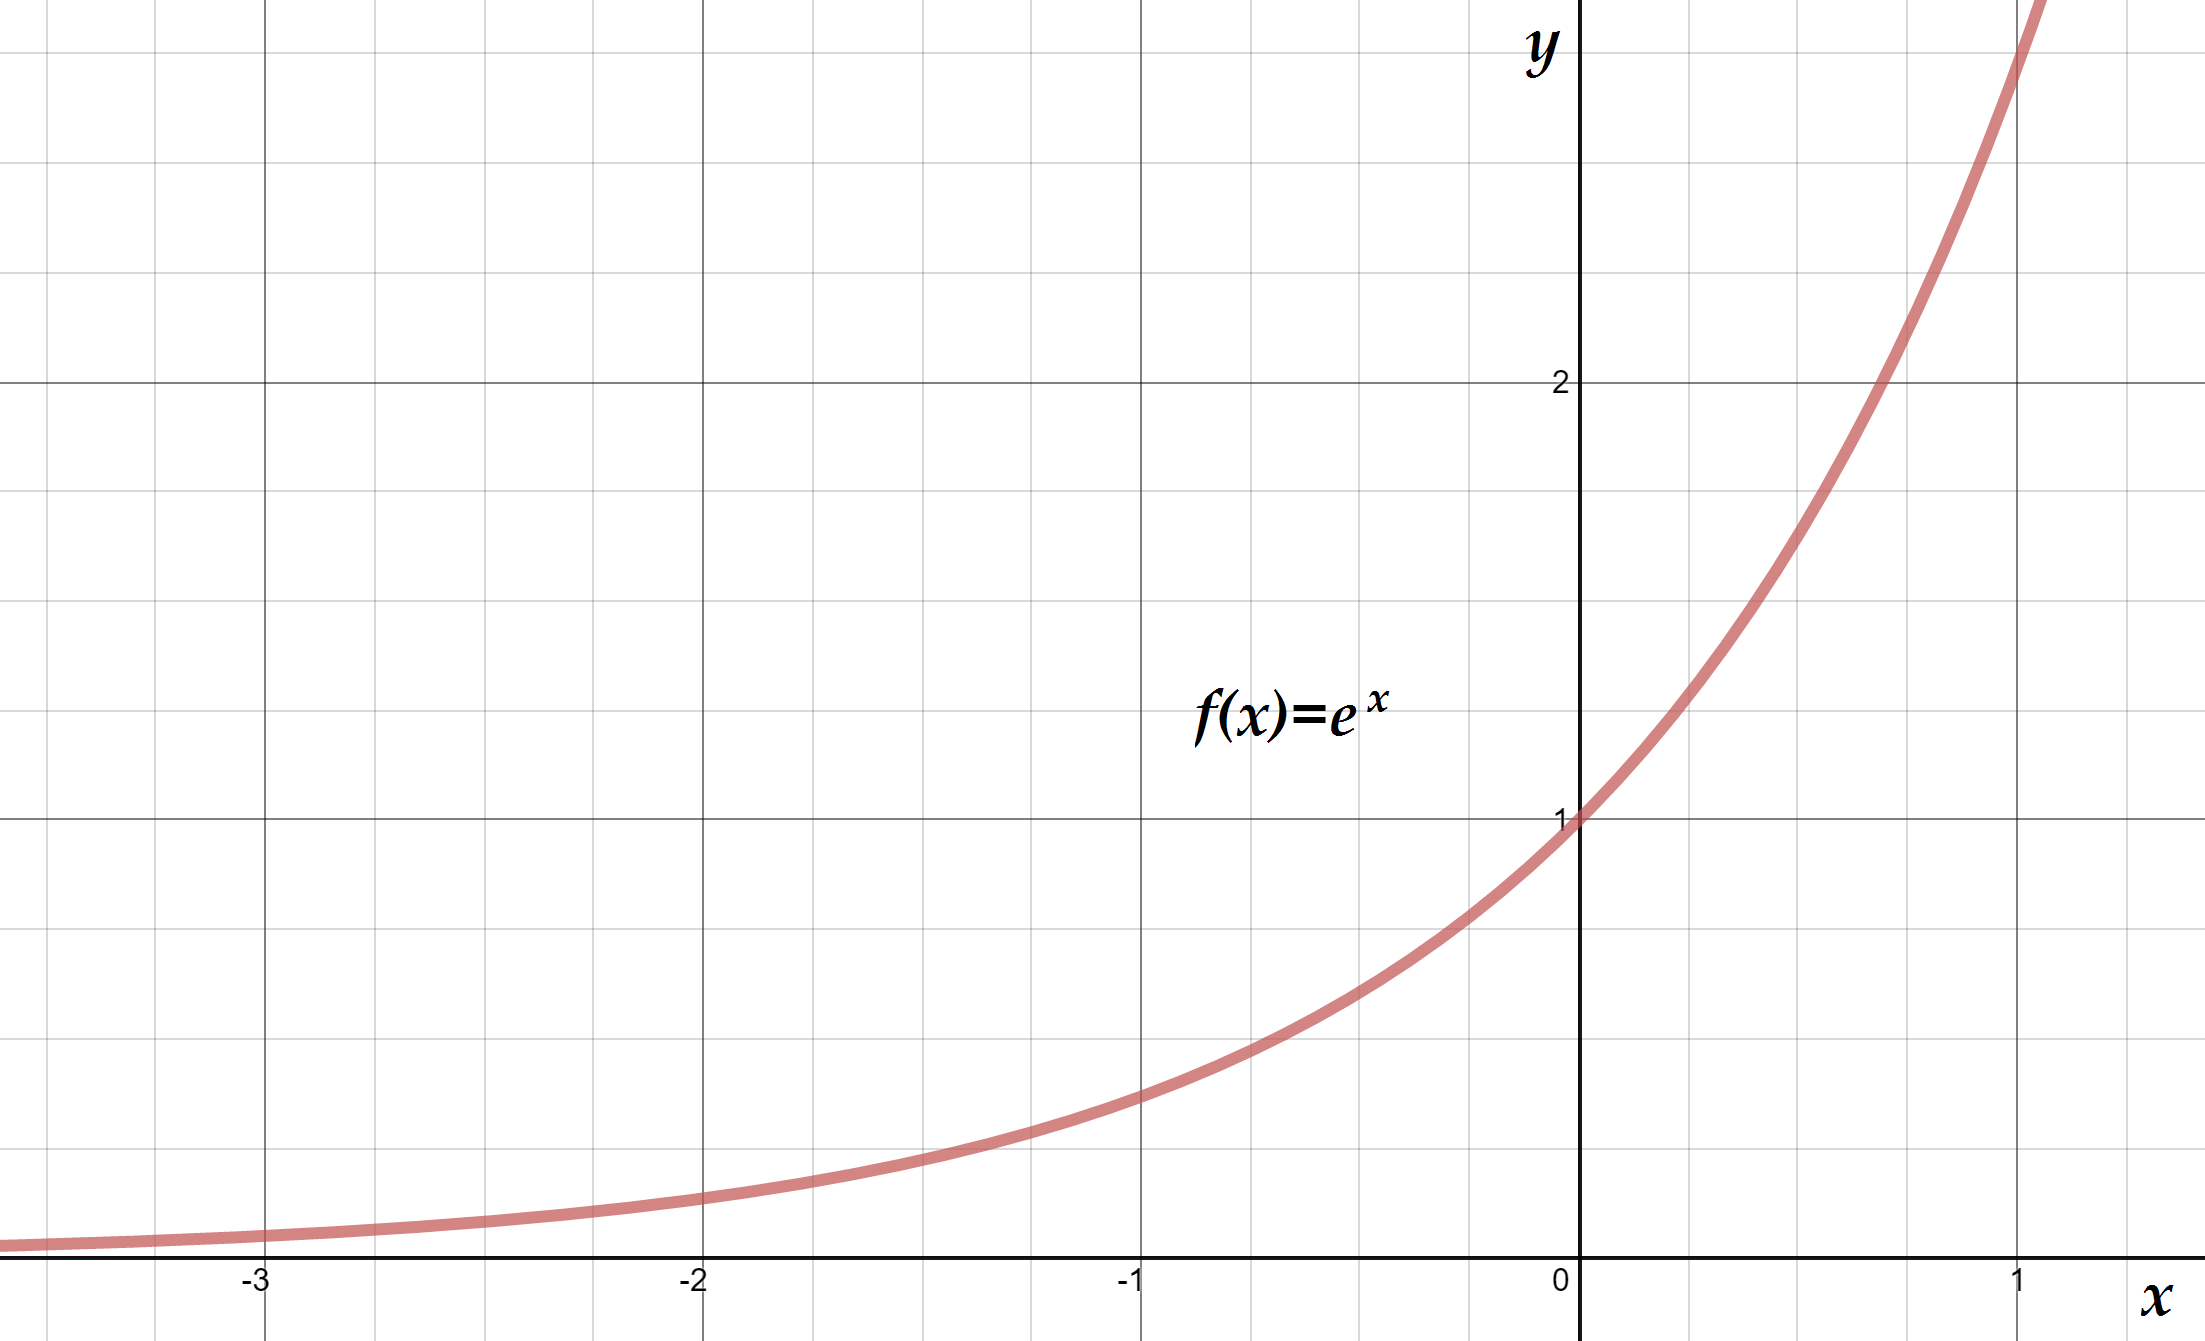
\includegraphics[scale=0.2]{expFunction}

{\footnotesize Exponential function drawn using \url{https://www.desmos.com/calculator}.}
\end{center}
\end{itemize}
\end{frame}

% % %
\begin{frame}
\begin{itemize}
\item Suppose $a,b\in\R$.  Then $e^{a+b}=e^a\cdot e^b$ implies $E(a+b)=E(a)\cdot E(b)$, the requirement for $E$ to be a group homomorphism.
\end{itemize}

\smallGap
Now we check $E$ is one-to-one.  Suppose there exist $a,b\in \R$ such that $E(a)=E(b)$.  Then 
\begin{align*}
e^a &= e^b \\
\implies \ln{(e^a)} &= \ln{(e^b)} \\
\implies a &= b,
\end{align*}
as required.
\end{frame}

% % %
\begin{frame}
%\smallGap
Finally, we must check $E$ is onto; if $x\in\R^+$ then we must show there exists $a\in\R$ such that $E(a)=x$.  One common technique is to define an \vocab{inverse} function for $E$.  Define
\begin{align*}
L:\R^+ &\to \R \\
x &\mapsto \ln x.
\end{align*}

\smallGap
If we put $a=\ln x$ for fixed $x\in\R^+$ then 
\[
E(a)=E(\ln x)=e^{\ln x}=x
\]
and we are done -- provided $L$ is well-defined.
\end{frame}

% % %
\begin{frame}
%\smallGap
Again, from Precalculus, we know the natural logarithm function is well-defined (see figure below); log algebra then shows for $x,y\in\R^+$, $\ln{(xy)}=\ln x+\ln y$, meaning $L(xy)=L(x)+L(y)$ and hence $L$ is a group homormorphism. 

\begin{center}
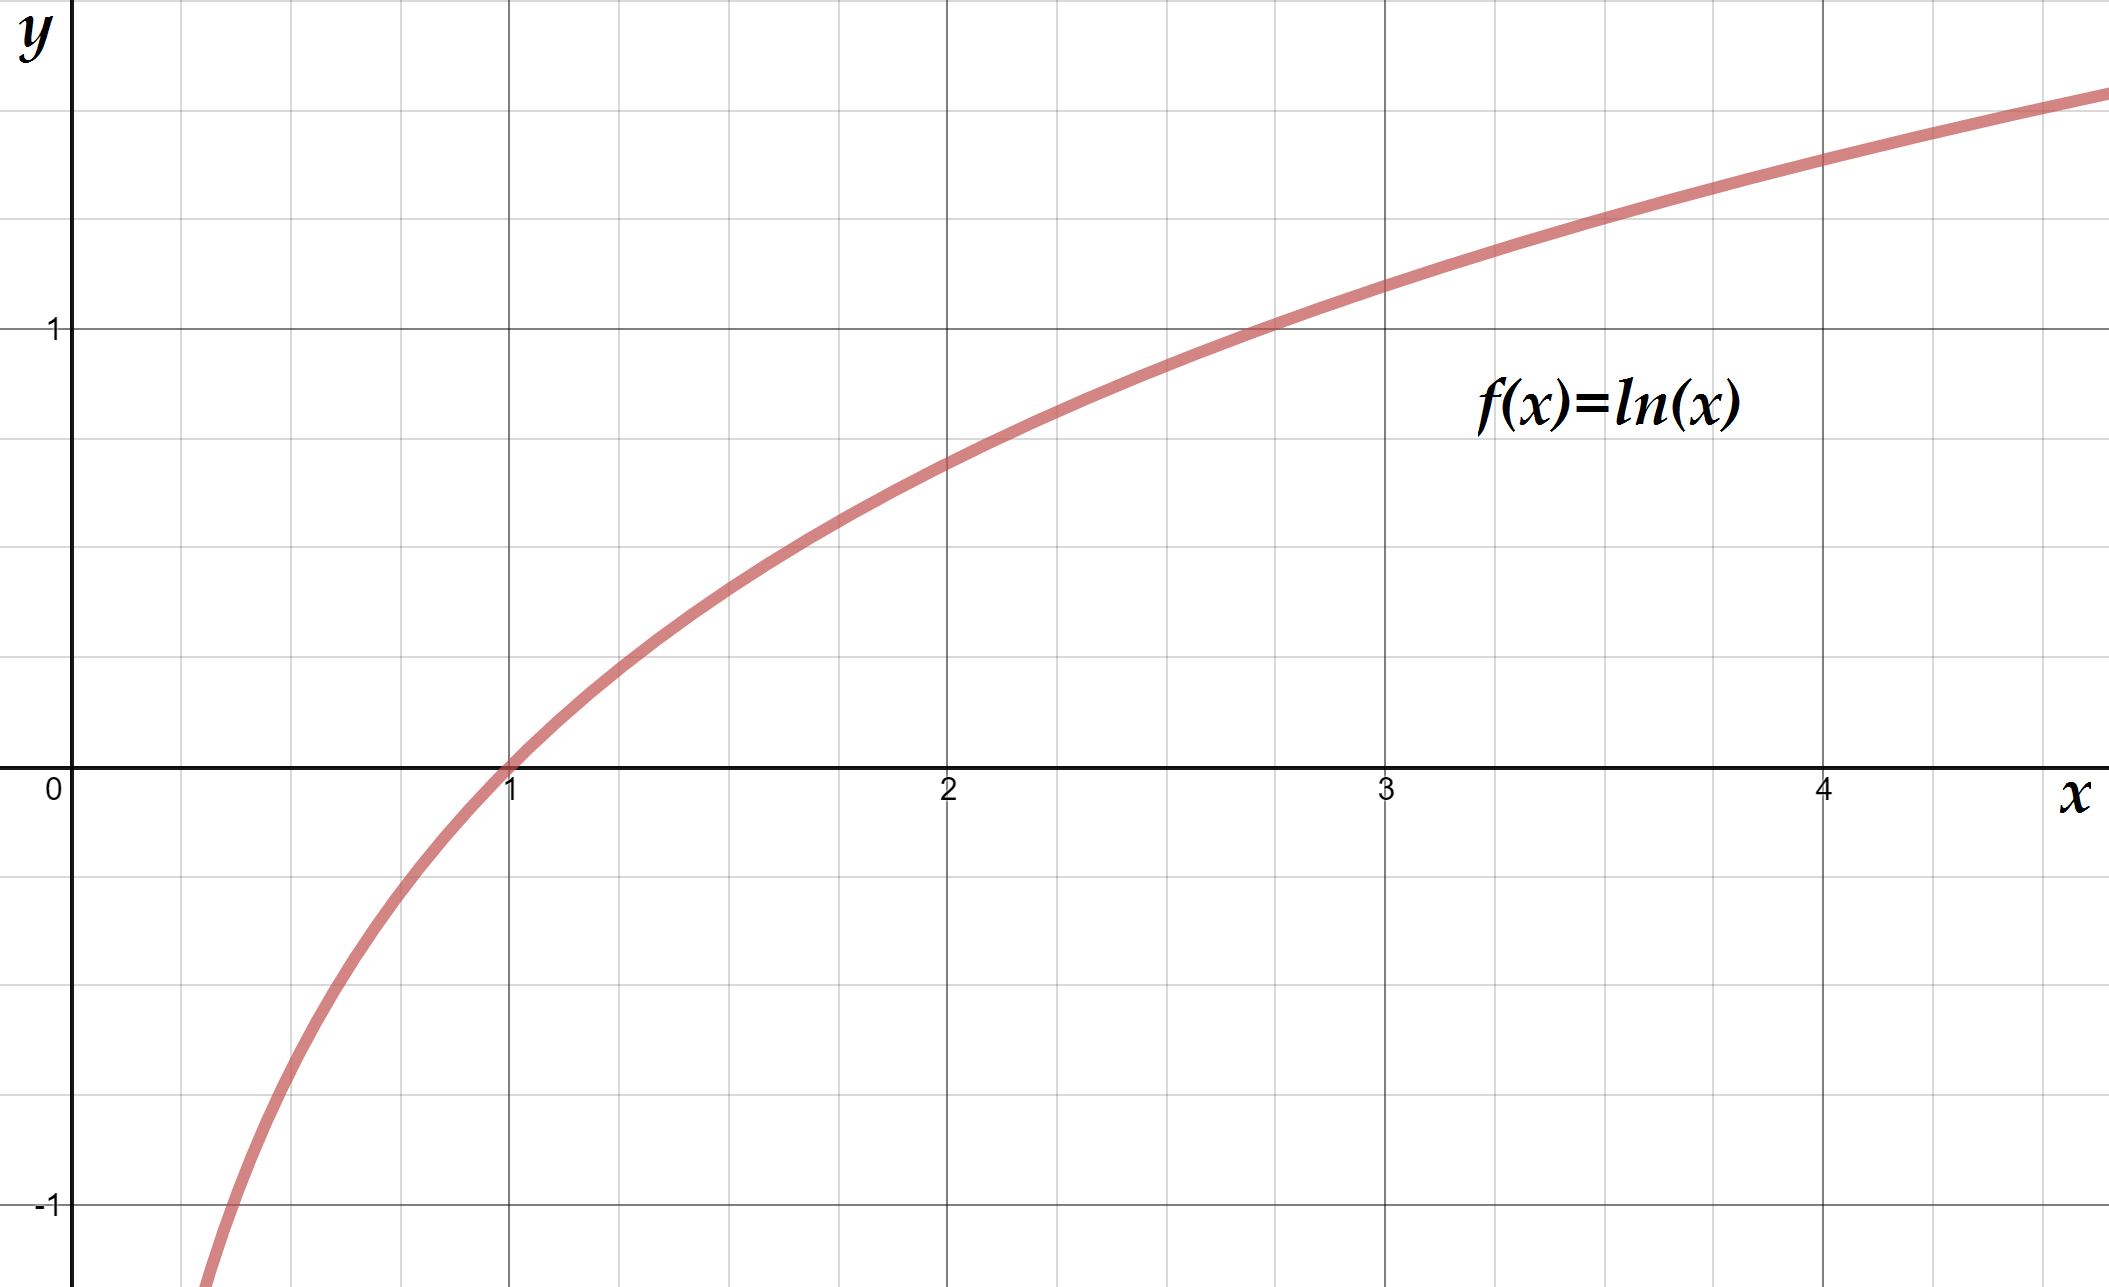
\includegraphics[scale=0.2]{lnFunction}

{\footnotesize Natural logarithm function drawn using \url{https://www.desmos.com/calculator}.}
\end{center}
\qed

%{\bf REMARK ABOUT RELATIONSHIP BETWEEN ADDITIVE AND MULTIPLICATIVE OPERATIONS}
\end{frame}

% % %
\begin{frame}[c]
\begin{prop}\label{prop:homomorphismIdentities}
Let $\varphi: G\to H$ denote a group homomorphism where the identities of $G$ and $H$, respectively, are $1_G$ and $1_H$.  Then $\varphi(1_G)=1_H$.

\qed
\end{prop}
%\begin{proof}
%{\bf PROOF}
%\end{proof}
%\end{frame}
%
% % %
%\begin{frame}

\smallGap
\begin{exe}\label{exe:homomorphismIdentities}
Verify Proposition \ref{prop:homomorphismIdentities} for Example \ref{ex:exponentialFunction}.
\end{exe}
\end{frame}

% % %
\begin{frame}
\begin{prop}\label{prop:relativelyPrime}
Let $p$ and $q$ be relatively prime numbers.  Then
\[
\Z/p\Z\times \Z/q\Z \cong \Z/pq\Z.
\]
\qed
\end{prop}

\smallGap
\begin{exe}\label{exe:relativelyPrime}
Prove Proposition \ref{prop:relativelyPrime}.
\end{exe}

\smallGap
\begin{exe}[cf. Problem 64]\label{exe:prob64}
Prove $\Z/2\Z\times \Z/4\Z \ncong \Z/8\Z$.
\end{exe}
\end{frame}

% % % % %
\subsection[\subsecname]{Kernels and images}\label{subsec:kernelsAndImages}
% % %
\begin{frame}{\subsecname}
One can show (see Exercise \ref{exe:prob65}) that the image of a group homomorphism is a subgroup of the target.  The source also has an important related subgroup.      
\begin{dfn}
Let $\varphi:G\to H$ denote a group homomorphism where $1_G$ and $1_H$ are the respective identity elements in $G$ and $H$.
\begin{enumerate}[(a)]
\item The \vocab{kernel} of $\varphi$, denoted $\ker{(\varphi)}$, is the set of all elements in $G$ mapped to the identity in $H$:
\[
\ker{(\varphi)}:=\{g\in G\mid \varphi(g)=1_H\}
\]
\item The \vocab{image} of $\varphi$ is the set of all elements in $H$ of the form $\varphi(g)$ for some $g\in G$:
\[
\image{(\varphi)}:=\{h\in H\mid h=\varphi(g)\text{ for some $g\in G$}\}.
\]
\end{enumerate}
\end{dfn}
\end{frame}

% % % 
%\begin{frame}{}{}
%{\bf EXAMPLE OF THE KERNEL AS A ZERO-SET}
%\end{frame}

% % %
\begin{frame}[c]
\begin{exe}[cf. Problem 65]\label{exe:prob65}
Let $\varphi:G\to H$ denote a group homomorphism.  Prove $\ker{\varphi}< G$ and $\image{\varphi}< H$.
\end{exe}
\end{frame}

% % %
\begin{frame}
\begin{ex}\label{ex:ZmodnZ}
This example motivates the content of Section \ref{sec:2p7quotientGroups}.  Define
\begin{align*}
\varphi:\Z &\to \Z_n \\
m &\mapsto m\mod n
\end{align*}
where $m\mod n$ is the remainder of $m$ upon division by $n$.
\end{ex}
\begin{que}
Why is $\varphi$ a well-defined function?
\end{que}

\smallGap
\textbf{Claim.} $\varphi$ is a (group) homomorphism.

%\smallGap
\end{frame}

% % % 
\begin{frame}
\pf  
Suppose $m_1,m_2\in\Z$.  By the Division Algorithm, there exist unique integers $q$ and $r$, with $0\leq r<n$, such that 
\begin{align*}
(m_1+m_2) &= nq+r \\
\implies r&= (m_1+m_2) -nq \\
	&\equiv (m_1+m_2) \mod n \\
	&= \varphi(m_1+m_2).
\end{align*}

\smallGap
Apply the Division Algorithm to $m_1,m_2$ as well, so that there exist unique integers $q_1,q_2$ and $r_1,r_2$, with $0\leq r_1,r_2<n$, such that 

\vspace{-0.75pc}
\begin{tabular}{p{0.4\textwidth}p{0.4\textwidth}}
{\begin{align*}
	m_1 &= nq_1+r_1 \\
	\implies r_1&= m_1 -nq_1 \\
	&\equiv m_1\mod n \\
	&= \varphi(m_1).
\end{align*}
} 
& {\begin{align*}
	m_2 &= nq_2+r_2 \\
	\implies r_2&= m_2 -nq_2 \\
	&\equiv m_2 \mod n \\
	&= \varphi(m_2).
\end{align*}
}
\end{tabular}
\end{frame}

% % %
\begin{frame}{}{}
Now apply the Division Algorithm to get unique integers $p,s$, with $0\leq s<n$ such that
\begin{align*}
np+s &= \left(\varphi(m_1)+\varphi(m_2)\right)\equiv s\mod n \\
	&= (m_1-nq_1)+(m_2-nq_2) \\
	&= (m_1+m_2)-n(q_1+q_2)
\end{align*}
by associativity.  Rearranging,
\[
m_1+m_2 = s+n(p+q_1+q_2).
\]
The uniqueness condition of the Division Algorithm says that $s=r$, because $0\leq s<n$.  Therefore
\[
\varphi(m_1+m_2)=r=s\equiv s\mod n=\varphi(m_1)+\varphi(m_2).
\]
\qed
\end{frame}

% % %
\begin{frame}
\textbf{Claim.} $\varphi$ is not injective.

\smallGap
\pf
We exhibit two distinct elements in $\Z$ with the same image.  Take $n-1\in\Z$ and $(n-1)+n\in\Z$.  Note, from Definition \ref{dfn:ZmodnZ}, $n\neq 0$, so $n-1\neq (n-1)+n$.  Since $n-1<n$, we have
\[
\varphi{(n-1)}=n-1\mod n=n-1.
\]
By the uniqueness condition in the Division Algorithm, we have
\begin{align*}
\varphi{\left((n-1)-n\right)} &= (n-1)+n(-1) \\
	&= (n-1)\mod n \\
	&= n-1.
\end{align*}
\qed
\end{frame}

% % %
\begin{frame}[c]
\textbf{Claim.} $\varphi$ is surjective.

\smallGap
\pf
$\Z/n\Z$ consists of non-negative integers strictly less than $n$, which are also in $\Z$.  If $m\in\Z/n\Z$, then 
\[
m=m\mod n=\varphi(m).
\]
\qed
\begin{que}
What are $\ker{(\varphi)}$ and $\image{(\varphi)}$?
\end{que}
\end{frame}

\begin{comment}
% % % % %
\answerKey
% % %
\begin{frame}{\subsecname}
\exeSol[(cf. Problem 62)]{exe:detExample}}
\end{frame}

% % %
\begin{frame}
\exeSol{exe:homomorphismIdentities}
\end{frame}

% % %
\begin{frame}
\exeSol{exe:relativelyPrime}
\end{frame}

% % %
\begin{frame}
\exeSol[(cf. Problem 64)]{exe:prob64}
\end{frame}

% % %
\begin{frame}
\exeSol[(cf. Problem 65)]{exe:prob65}
\end{frame}

\end{comment}
% % % % % % % % % %
\end{document}